\section{\textbf{Atomic MRSW Register}}
% -------------------------------------------------------------------------------- %
\subsection{Particular Case}
\par
The characteristics of this type of register are:
\begin{itemize}
\item It should never happen that $R^{i} \rightarrow W^{i}$
\item It should never happen that for any ${j}$, ${W^{i} \rightarrow W^{j} \rightarrow R^{j}}$
\item If ${R^{i} \rightarrow R^{j}}$ then ${i \leq j}$
\end{itemize}
The book proposes to do this by using multiple SRSW registers.
% -------------------------------------------------------------------------------- %
\subsection{Solution}
The algorithm then requires a 2 dimensional table. When a writer decides to
update the register, it has to update the values in cells $A[i][i]$, where $i$
is the thread id. Apart from writing the value, it has to also update the cell
with a timestamp. 
\par
In the other hand, when a reader wants to read from the register, it checks the
timestamp of the cell $A[i][i]$. After that, it has to check other cells in the
same column (ie, cells $A[x][i]$) to see if there has been an update in between.
That is done by comparing the timestamps. If there is a newer timestamp, the
reader has then to update all cells in its row (ie $A[i][x]$). This is the way
to indicate subsequent readers which version of the value has the previous
reader retrieved.
\par
It is easy to see that the first property is satisfied because there is no way
to read a future value. In order to read a value, this value has to be written
before.
\par
The second property is also satisfied because when a reader reads the value, it
reads the one with the most recent timestamp by scaning the timestamps in its
corresponding column. This reader also helps subsequent readers by updating all
cells in its row. Forcing property 3 to be satisfied as well.
\par
% -------------------------------------------------------------------------------- %
\subsection{Experiment Description}
\par 
The two test cases presented demonstrates the same as previous examples so we
will not describe the experiment further. 
\par
These are the details of the system we used to run the experiments:
\begin{itemize}
\item Processor: Intel Core i5 @2.5 GHz. 2 Cores.
\item L2 Cache per Core: 256 KB
\item L3 Cache: 3 MB
\item System Memory: 16 GB
\end{itemize}
% -------------------------------------------------------------------------------- %
\subsection{Sample Results}
As in previous examples, we identified that the test fails from time to time.
Figure \ref{fig:AtomicMRSW00} shows the output when the failure is seen.
\par
\par
\begin{figure}[h]
  \centering
  \includegraphics[width=13cm]{AtomicMRSW00.png}
  \caption{First type of failure}
  \label{fig:AtomicMRSW00}
\end{figure}
\par
Again, the fix for these failures was to reset the thread ids.
\par
\begin{figure}[h]
  \centering
  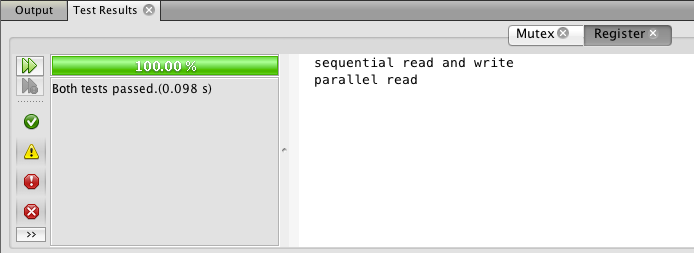
\includegraphics[width=13cm]{AtomicMRSW01.png}
  \caption{Output after fix}
  \label{fig:AtomicMRSW01}
\end{figure}
\par
\begin{figure}[h]
  \centering
  \includegraphics[width=13cm]{AtomicMRSW02.png}
  \caption{Output after fix of threadIds}
  \label{fig:AtomicMRSW03}
\end{figure}
\par
% -------------------------------------------------------------------------------- %
\subsection{Interpretation}
\par
In this experiment we observed a way of implementing MRSW registers. We saw
that, at least in the processor we used, the algorithm seems to work correctly.
\par
It would have been great, though, to also have test cases that demonstrate that this
particular register satisfies property 3 which is the one that makes it
different from the Safe version.
% -------------------------------------------------------------------------------- %
